\documentclass[11pt,a4paper]{article}
\usepackage[margin=2.2cm]{geometry}
\usepackage{amsmath,amssymb,graphicx,booktabs,natbib,xcolor,longtable}
\usepackage[colorlinks=true,linkcolor=blue!55!black,citecolor=blue!55!black,
            urlcolor=blue!45!black]{hyperref}
\usepackage{microtype}
\bibliographystyle{plainnat}
\setlength{\parskip}{2pt}
\newcommand{\Ke}{K_{\mathrm{e}}}
\newcommand{\Kini}{K_{\mathrm{ini}}}
\newcommand{\zi}{z_{\mathrm{i}}}
\newcommand{\ergs}{\ \mathrm{erg\,s^{-1}}}
\newcommand{\cmt}{\ \mathrm{cm^{-3}}}

\title{\bf Little Red Dots as cosmic-ray electron sources:\\
       literature status, competing hypotheses, and a recipe for\\
       estimating the index and normalization of their electron spectrum}
\author{Report prepared for L.\ Carvalho \\
        \small companion to \texttt{manuscript/manuscript.tex}
        (cosmic-ray electrons in the IGM, $z=5.5$--$20$)}
\date{31 August 2026}

\begin{document}
\maketitle

\begin{abstract}
\noindent
This report answers four questions in order. \textbf{(1)} It surveys the Little
Red Dot (LRD) literature to the end of August 2026. \textbf{(2)} It lists the
nine hypotheses currently on the table for what LRDs are. \textbf{(3)} It
identifies which of those objects can accelerate cosmic rays and gives an
explicit, closed recipe for estimating the index $s$ and the normalization $K$
of a power-law cosmic-ray electron spectrum $N(\gamma)=K\gamma^{-s}$, along both
a forward (energetic) and an inverse (radio-limit) route, with a worked fiducial.
\textbf{(4)} Every algebraic step is verified symbolically with
\textsc{SymPy} (\texttt{verify\_algebra.py}); every number is produced by
\texttt{lrd\_cr\_numbers.py}, which also reproduces Table~3 of the companion
manuscript to $0.14\%$. The central finding is that the radio non-detections of
LRDs do \emph{not} constrain their cosmic-ray electron content, because
inverse-Compton losses in the dense cocoon suppress synchrotron emission by a
factor $1+U_{\mathrm{rad}}/U_B \sim 10^2$--$10^5$; the constraint they do
provide is three orders of magnitude weaker than the fiducial prediction.
Folding the escaping electrons through the cascade yield table of the companion
manuscript gives $2\times10^{-6}$--$10^{-4}$ ionizations per hydrogen atom and
$\Delta T\sim0.1$--$18\ \mathrm{K}$ for plausible parameters.
\end{abstract}

% =====================================================================
\section{Scope and rules}
% =====================================================================
This report follows the conventions of the companion manuscript: every physical
statement is attributed to a real publication, cited in \textsc{Bib}\TeX{} form,
with a free-access link collected in Sect.~\ref{sec:refs}; figures are produced
by \texttt{.py} files in this directory; and no astrophysical hypothesis is
adopted without it being flagged as such. Assumptions that are mine rather than
the literature's are marked \textbf{[A]} throughout.

% =====================================================================
\section{The recent literature on Little Red Dots}
\label{sec:lit}
% =====================================================================
LRDs were defined observationally as compact, red, high-redshift sources with
``V-shaped'' rest-frame UV--optical spectral energy distributions and, very
often, broad Balmer emission lines
\citep{Matthee2024,Labbe2025,Greene2024,Kocevski2025}. They are abundant:
$n\simeq10^{-5}$--$10^{-4}\ \mathrm{cMpc^{-3}}$ at $z\simeq5$
\citep{Matthee2024,Akins2025}, orders of magnitude above the luminous-quasar
density at the same epoch. \citet{Loiacono2026} show there is no significant
evolution in the abundance of LRDs with
$L_{\mathrm{bol}}\gtrsim3\times10^{44}\ergs$ over $z>2$, reaching
$n = 3.4^{+5.6}_{-2.4}\times10^{-5}\ \mathrm{Mpc^{-3}}$ at cosmic noon.

Three observational facts drive the whole debate. First, LRDs are extremely
X-ray weak: \citet{Ananna2024} and \citet{Tortosa2026} find non-detections
individually and in stacks, and \citet{Sacchi2025} stacked $55$ LRDs in the
\emph{Chandra} Deep Fields for nearly $400\ \mathrm{Ms}$ and still recovered
nothing, which rules out a population of unobscured, intrinsically luminous
super-Eddington accretors. Second, they are radio silent:
\citet{Perger2025} stacked $919$ LRDs in VLASS and FIRST and found no emission
above $3\sigma$ noise levels of $\sim\!11$ and $\sim\!18\ \mu\mathrm{Jy\,
beam^{-1}}$ respectively, while \citet{Akins2025} stacked $434$ LRDs in
COSMOS-Web with MeerKAT ($1.4\ \mathrm{GHz}$) and the VLA ($3\ \mathrm{GHz}$)
and derived a radio-loudness upper limit $R_{4400}=L_{5\,\mathrm{GHz}}/
L_{4400\,\text{\AA}}\le10$ \citep[in the sense of][]{Kellermann1989};
\citet{Mazzolari2026} collect all the stacking attempts and note that the
deepest reach $0.5$--$0.1\ \mu\mathrm{Jy}$ at $z\sim5$--$6$. Third, the best
spectra show enormous Balmer breaks together with Balmer \emph{absorption}
\citep{Naidu2025,Rusakov2026}, which no ordinary stellar population produces.

Two 2026 results reframe the field. \citet{Rusakov2026}, in \emph{Nature},
argue that the line broadening is caused by electron scattering in a dense
ionized cocoon of light-day scale rather than by Doppler motion, so that the
intrinsic line cores imply $M_{\mathrm{BH}}=10^{5-7}\,M_\odot$ --- two orders of
magnitude below previous estimates --- and the cocoon simultaneously explains
the weak radio and X-ray signatures. \citet{Barrufet2026} find that the LRD
fraction rises strongly with H$\alpha$ luminosity, which disfavours a simple
orientation-based unification with ``little blue dots'' and instead supports
gas-cocoon models in which column density drives the transition. Finally,
\citet{Rodriguez2026} report the first radio-bright local LRD analogue, J2048 at
$z=0.4332$, with $S_{3\,\mathrm{GHz}}=3.0\pm0.2\ \mathrm{mJy}$,
$\alpha=-0.39\pm0.04$ and $L_{\mathrm{radio}}=1.2\times10^{41}\ergs$, and
propose that inverse-Compton cooling by ultraviolet photons dims the synchrotron
emission of the high-redshift population while leaving the mechanical output
intact. That proposal is the pivot of Sect.~\ref{sec:est}.

% =====================================================================
\section{The hypotheses currently being debated}
\label{sec:hyp}
% =====================================================================
Table~\ref{tab:hyp} lists the nine distinct proposals that are alive in the
literature as of August 2026, grouped by what the central object is.

\begin{table}[t]\centering\small
\caption{Competing hypotheses for the nature of Little Red Dots. ``Engine'' is
the object that supplies the luminosity. The two right-hand columns anticipate
Sect.~\ref{sec:which}.}
\label{tab:hyp}
\begin{tabular}{@{}p{0.30\textwidth}p{0.30\textwidth}cc@{}}
\toprule
Hypothesis & Engine and key claim & Refs. & CR site? \\
\midrule
\textbf{H1} Obscured / dust-reddened AGN &
Standard SMBH with a dusty screen; the original reading &
\citealt{Matthee2024,Labbe2025,Kocevski2025} & yes \\
\addlinespace
\textbf{H2} Black-hole star (BH$^\star$) &
SMBH inside a dust-free, dense, turbulent ``atmosphere'' that makes the Balmer
break and absorption &
\citealt{Naidu2025} & yes \\
\addlinespace
\textbf{H3} Dense ionized cocoon around a low-mass SMBH &
Electron scattering, not Doppler motion, broadens the lines;
$M_{\mathrm{BH}}=10^{5-7}M_\odot$, near-Eddington &
\citealt{Rusakov2026,Barrufet2026} & yes \\
\addlinespace
\textbf{H4} Super-Eddington / supercritical accretion &
Puffed-up, self-shielding disc; intrinsic X-ray weakness and the Balmer break
come from the accretion flow itself &
\citealt{Liu2025,LiuJR2026} & yes \\
\addlinespace
\textbf{H5} Supermassive analogue of SS\,433 &
Hyper-Eddington microquasar physics scaled up, viewed at high inclination;
LBDs are the low-inclination counterparts &
\citealt{Zhou2026} & \textbf{yes} \\
\addlinespace
\textbf{H6} Intermediate-mass super-Eddington engine
($\eta$\,Car / Type\,IIn analogue) &
Slow dense wind forms a pseudo-photosphere; fast winds crash into it and
generate shocks; $M<10^{5}M_\odot$ &
\citealt{Naidu2026} & \textbf{yes} \\
\addlinespace
\textbf{H7} Direct-collapse black hole (DCBH) &
Compressionally heated, collisionally ionized accretion flow onto a heavy seed
in a pristine atomic-cooling halo &
\citealt{Pacucci2026} & marginal \\
\addlinespace
\textbf{H8} Quasi-star / supermassive star &
An SMBH seed inside a convective envelope radiating a $T\sim5000\ \mathrm{K}$
black body; or a hierarchically nested supermassive star trapping a nuclear
star cluster &
\citealt{Gentile2026,AmaroSeoane2026,Shi2026} & marginal \\
\addlinespace
\textbf{H9} Compact star-forming galaxy (no AGN required) &
Ultra-compact stellar cores, $R_{\mathrm{eff}}<300\ \mathrm{pc}$,
$V_{\mathrm{circ}}>500\ \mathrm{km\,s^{-1}}$; reproduces the break and the UV
slope but not the reddest continua or the broadest lines &
\citealt{Roy2026,Vaida2026} & \textbf{yes} \\
\bottomrule
\end{tabular}
\end{table}

Two remarks on the state of the debate. The evidence has moved decisively
against H1 in its pure form: the dust reservoirs are too small
\citep{Rusakov2026,Naidu2025} and the X-ray weakness is too severe
\citep{Sacchi2025,Tortosa2026}. And H9 in its pure form is disfavoured because
broad Balmer lines and Balmer absorption are not produced by ordinary
H\,\textsc{ii} regions, although \citet{Roy2026} show that ultra-compact
galaxies reproduce a real subset of the properties, which is why most reviews
now describe LRDs as a mixed or hybrid population \citep{Vaida2026}.
H3, H4, H5 and H6 are variations on a single physical picture --- a
super-Eddington engine buried in a dense, scattering-dominated envelope --- and
differ mainly in the mass of the engine and the geometry of the outflow.

% =====================================================================
\section{Which of them can accelerate cosmic rays}
\label{sec:which}
% =====================================================================
A site accelerates cosmic rays if it has (i) a converging flow or a
reconnecting field to energize particles, (ii) enough magnetic confinement to
keep them there while they gain energy, and (iii) losses slow enough that the
gain wins. Applying that filter to Table~\ref{tab:hyp} isolates four sites,
which are the four columns of Table~\ref{tab:sites}.

\begin{description}
\item[(i) Jet / polar funnel.] Present in H1--H5. \citet{Kuze2026} build the
only explicit particle-acceleration model of an LRD to date: relativistic jets
and outflows launched from the black hole propagate through low-density polar
funnels inside the envelope, and dissipate there. Their fiducial parameters are
$M_{\mathrm{BH}}=10^{6.5}M_\odot$, envelope mass $10^{6.5}M_\odot$,
dissipation radius $r_{\mathrm{dis}}=10^{16}\ \mathrm{cm}$, jet Lorentz factor
$\Gamma_j=2$, magnetic energy fraction $\epsilon_B=0.01$, gyrofactor $\eta=10$,
a proton acceleration efficiency $\epsilon_p=0.1$ and an
$\varepsilon_p^{-2}$ injection spectrum; they quote a comoving field
$B'\simeq1.3\times10^{2}\ \mathrm{G}$ for a strongly collimated funnel.

\item[(ii) Fast wind driving into the dense envelope.] This is the core of H6:
``the engine may also launch fast winds that crash into the existing envelope to
generate shocks'' \citep{Naidu2026}. It is observationally supported ---
\citet{Korber2026} report direct evidence for a fast AGN-driven outflow in a
$z=6.64$ LRD host with a kinetic luminosity $\sim\!10^{43}\ergs$, and
\citet{Rodriguez2026} argue for powerful mechanical outflows in the local
analogue. H5 makes the same prediction by construction, since SS\,433's
jets inflate the W50 nebula.

\item[(iii) Accretion-disc corona.] Present in H1--H4, H7. Magnetic reconnection
in a hot corona does accelerate particles, but as Table~\ref{tab:sites} shows
the radiation energy density at $10\,R_g$ exceeds the magnetic energy density by
$3\times10^{5}$, so the maximum electron energy collapses to $\sim\!10\
\mathrm{GeV}$ and nothing escapes. This site is a heater, not a cosmic-ray
source.

\item[(iv) Host-galaxy supernovae.] Present in H9 and in the hybrid readings of
H3 and H6. This is the textbook cosmic-ray channel \citep{Bell1978,
BlandfordOstriker1978,Drury1983}; the relevant point here is that
\citet{Mazzolari2026} show the deepest SKAO observations will test exactly this
scenario, probing $\mathrm{SFR}\sim5$--$50\ M_\odot\,\mathrm{yr^{-1}}$ at
$z\sim5$--$6$.
\end{description}

H7 and H8 are marked ``marginal'' because their defining feature is a
\emph{quasi-hydrostatic, convective, radiation-dominated} envelope
\citep{Pacucci2026,Gentile2026,AmaroSeoane2026}: there is no supersonic
converging flow, so first-order Fermi acceleration has nothing to work with,
even though the envelope is magnetized.

% =====================================================================
\section{How to estimate the cosmic-ray electron spectrum}
\label{sec:est}
% =====================================================================
Write the steady-state electron spectrum inside the source as
\begin{equation}
  N(\gamma)\,\mathrm d\gamma = K\,\gamma^{-s}\,\mathrm d\gamma ,
  \qquad \gamma_{\min}\le\gamma\le\gamma_{\max}.
  \label{eq:pl}
\end{equation}
Estimating it means fixing four things: the index $s$, the two ends
$\gamma_{\min},\gamma_{\max}$, and the normalization $K$. Everything below is
verified symbolically in \texttt{verify\_algebra.py}.

\subsection{The index}
\label{sec:index}
There are two independent routes, and they should be used as a consistency
check on each other.

\paragraph{Theory (forward).} For diffusive shock acceleration the momentum
distribution is $f(p)\propto p^{-q}$ with $q=3r/(r-1)$, $r$ the compression
ratio \citep{Bell1978,BlandfordOstriker1978,Drury1983}. Since
$N(E)\,\mathrm dE\propto p^{2}f(p)\,\mathrm dp$, the energy index is
\begin{equation}
  s=\frac{r+2}{r-1},
  \qquad
  r=\frac{(\gamma_{\mathrm{ad}}+1)\mathcal M^{2}}
         {(\gamma_{\mathrm{ad}}-1)\mathcal M^{2}+2}
  \;\Longrightarrow\;
  s(\mathcal M)=\frac{2(\mathcal M^{2}+1)}{\mathcal M^{2}-1}
  \quad (\gamma_{\mathrm{ad}}=5/3),
  \label{eq:dsa}
\end{equation}
so $s\to2$ for a strong shock and $s=2.17,\,2.50,\,3.33$ for
$\mathcal M=5,\,3,\,2$. The wind shock of site (ii) has
$\mathcal M\simeq198$ against $10^{4}\ \mathrm{K}$ gas
(Table~\ref{tab:sites}), i.e.\ $r=4.000$ and $s=2.000$ to four figures. This is
why \citet{Kuze2026} adopt $\varepsilon^{-2}$ for the protons; the same argument
fixes the electrons. Mildly relativistic and oblique shocks steepen this to
$s\simeq2.2$--$2.4$, and supernova remnants empirically sit at $s\simeq2.1$--$2.4$.

\paragraph{Observation (inverse).} For an optically thin synchrotron source the
flux index $\alpha$ (with $S_\nu\propto\nu^{\alpha}$) and $s$ are locked:
\begin{equation}
  \alpha = -\frac{s-1}{2}
  \qquad\Longleftrightarrow\qquad
  s = 1-2\alpha .
  \label{eq:alpha}
\end{equation}
Equation~(\ref{eq:alpha}) is verified in \texttt{verify\_algebra.py} by two
independent routes (a $\delta$-function kernel and the exact $F(\nu/\nu_c)$
kernel). \emph{Caveat}: applied to the only LRD analogue with a measured radio
slope, $\alpha=-0.39\pm0.04$ for J2048 \citep{Rodriguez2026}, this returns
$s=1.78$, which is flatter than any shock can produce --- and the authors
themselves attribute the slope to \emph{optically thick} synchrotron, for which
Eq.~(\ref{eq:alpha}) does not hold. This is the single most important practical
warning in this section: in an LRD, self-absorption and free--free absorption in
the cocoon corrupt the spectral index, so $s$ must come from theory and the
radio slope can only be used once the source is demonstrably optically thin.

\paragraph{Cooling break.} Wherever radiative losses beat escape, the
steady-state solution of $\partial_\gamma(\dot\gamma N)=-Q$ with
$\dot\gamma=-b\gamma^{2}$ and injection $Q\propto\gamma^{-s}$ is
\begin{equation}
  N(\gamma)=\frac{Q_0}{b\,(s-1)}\,\gamma^{-(s+1)},
  \qquad
  b=\frac{4\sigma_{\mathrm T}}{3m_ec}\,\bigl(U_B+U_{\mathrm{rad}}\bigr),
  \label{eq:cool}
\end{equation}
i.e.\ the index steepens by exactly one above
$\gamma_b=1/(b\,t)$. In an LRD cocoon $b$ is enormous and $\gamma_b$ is of order
unity, so the \emph{observable} population is the cooled one, with $s+1\simeq3$.

\subsection{The two ends of the spectrum}
$\gamma_{\min}$ is set by injection out of the thermal pool and is of order a
few; it matters only for $s>2$, where it controls the energy budget.
$\gamma_{\max}$ is the smaller of two limits, both verified symbolically:
\begin{align}
  \text{confinement (Hillas):}\quad
  &E_{\max}[\mathrm{eV}] = 299.79\,\beta\,B[\mathrm{G}]\,R[\mathrm{cm}],
  \label{eq:hillas}\\[2pt]
  \text{radiative burn-off:}\quad
  &E_{\max}=m_ec^{2}\sqrt{\frac{3\,e\,B}{4\,\eta\,\sigma_{\mathrm T}\,U_{\mathrm{tot}}}},
  \qquad U_{\mathrm{tot}}=U_B+U_{\mathrm{rad}},
  \label{eq:burnoff}
\end{align}
where $\eta\ge1$ is the gyrofactor (Bohm limit $\eta=1$;
\citealt{Kuze2026} take $\eta=10$). Equation~(\ref{eq:burnoff}) reduces, for
$U_{\mathrm{tot}}=U_B=B^{2}/8\pi$, to
$E_{\max}=m_ec^{2}\sqrt{6\pi e/(\eta\sigma_{\mathrm T}B)}\propto B^{-1/2}$, and
the corresponding \emph{synchrotron photon} energy is independent of $B$,
\begin{equation}
  E_\gamma^{\mathrm{burn}}=\frac{27}{8}\,\frac{m_ec^{2}}{\alpha_{\mathrm f}\,\eta}
  \simeq\frac{236\ \mathrm{MeV}}{\eta},
  \label{eq:burnphot}
\end{equation}
the familiar $\sim\!10^{2}\ \mathrm{MeV}$ synchrotron limit (the exact
coefficient depends on the convention adopted for $t_{\mathrm{acc}}$; ours is
$t_{\mathrm{acc}}=\eta E/eBc$). In an LRD, $U_{\mathrm{rad}}\gg U_B$, so
both $E_{\max}$ and $E_\gamma^{\mathrm{burn}}$ fall by
$\sqrt{U_B/U_{\mathrm{tot}}}$. This is the quantitative form of the
radio-dimming mechanism proposed by \citet{Rodriguez2026}.

\subsection{Normalization, route A: forward from the energy budget}
\label{sec:normA}
Integrating Eq.~(\ref{eq:pl}) over energy,
\begin{equation}
  U_e=\int_{\gamma_{\min}}^{\gamma_{\max}}K\gamma^{-s}\,\gamma m_ec^{2}\,\mathrm d\gamma
     =K m_ec^{2}\,
      \frac{\gamma_{\max}^{2-s}-\gamma_{\min}^{2-s}}{2-s}
  \;\xrightarrow[\;s\to2\;]{}\;
  K m_ec^{2}\ln\!\frac{\gamma_{\max}}{\gamma_{\min}},
  \label{eq:norm}
\end{equation}
the $s=2$ limit being the one that actually applies. The recipe is then three
steps:
\begin{enumerate}
\item \emph{Get the mechanical power $L_{\mathrm{mech}}$.} For the jet site,
      \citet{Kuze2026} set $L_j=L_{\mathrm{Edd}}=10^{44.6}\ergs$ for
      $M_{\mathrm{BH}}=10^{6.5}M_\odot$. For the wind site, use the measured
      outflow kinetic luminosity: \citet{Korber2026} give
      $\sim\!10^{43}\ergs$. For the stellar site, use
      $L_{\mathrm{mech}}\simeq10^{42}\,(\mathrm{SFR}/M_\odot\,\mathrm{yr^{-1}})\ergs$
      from the supernova rate.
\item \emph{Adopt an electron acceleration efficiency $\epsilon_e$}
      \textbf{[A]}. There is no LRD measurement of $\epsilon_e$;
      $\epsilon_e=0.01$--$0.1$ brackets what is used for shocks elsewhere, and
      \citet{Kuze2026} adopt $\epsilon_p=0.1$ for protons in this very system.
      Then $L_e=\epsilon_e L_{\mathrm{mech}}$.
\item \emph{Convert to $K$} through $U_eV=L_e\,t$, with
      $t=\min(t_{\mathrm{dyn}},t_{\mathrm{cool}})$ and $V$ the emitting volume:
      \begin{equation}
        K=\frac{L_e\,t}{V\,m_ec^{2}\ln(\gamma_{\max}/\gamma_{\min})}\quad(s=2).
      \end{equation}
\end{enumerate}

\subsection{Normalization, route B: inverse, from the radio non-detections}
\label{sec:normB}
Converting a flux limit to a luminosity requires the K-correction
\begin{equation}
  S_\nu=\frac{(1+z)^{1+\alpha}L_\nu(\nu_{\mathrm{obs}})}{4\pi D_L^{2}},
  \label{eq:kcorr}
\end{equation}
and the crucial step, which is where most of the physics sits, is that in fast
cooling only a fraction $U_B/(U_B+U_{\mathrm{rad}})$ of the electron power comes
out as synchrotron radiation, the rest being inverse-Compton:
\begin{equation}
  L_e = L_{\mathrm{sync}}\left(1+\frac{U_{\mathrm{rad}}}{U_B}\right).
  \label{eq:deboost}
\end{equation}
A synchrotron upper limit therefore translates into an electron-power upper
limit that is \emph{weaker} by $1+U_{\mathrm{rad}}/U_B$. If instead one has a
detection and wants the minimum energy content, the classical minimum-energy
condition follows from minimizing $U_e+U_B$ at fixed $L_{\mathrm{sync}}$ and
gives, exactly,
\begin{equation}
  \frac{U_B}{U_e}=\frac{s+1}{4}
  \qquad\bigl(=\tfrac34\ \text{for}\ s=2\bigr).
  \label{eq:equip}
\end{equation}

\subsection{Worked fiducial}
\label{sec:fid}
Table~\ref{tab:sites} evaluates the four sites for an LRD at $z=5$ with
$M_{\mathrm{BH}}=10^{6.5}M_\odot$ ($L_{\mathrm{Edd}}=3.98\times10^{44}\ergs$),
$L_{\mathrm{bol}}=10^{45}\ergs$ and an envelope of radius
$R=10^{16}\ \mathrm{cm}$ (3.9 light-days, matching the light-day scale of
\citealt{Rusakov2026}). All entries come from \texttt{lrd\_cr\_numbers.py}.

\begin{table}[t]\centering\small
\caption{The four candidate acceleration sites, evaluated for the fiducial LRD.
$f_{\mathrm{sync}}=U_B/(U_B+U_{\mathrm{rad}})$ is the fraction of the electron
power that emerges as synchrotron radiation. $E_{\max}$ from
Eqs.~(\ref{eq:hillas}) and (\ref{eq:burnoff}) with $\eta=1$.}
\label{tab:sites}
\begin{tabular}{@{}lrrrrrrr@{}}
\toprule
site & $B$ [G] & $U_B$ [erg\,cm$^{-3}$] & $U_{\mathrm{rad}}/U_B$ &
$s$ & $E_{\max}^{\mathrm{Hillas}}$ [eV] & $E_{\max}^{\mathrm{cool}}$ [eV] &
$f_{\mathrm{sync}}$ \\
\midrule
jet funnel  & $0.82$ & $2.6\times10^{-2}$ & $251$ & $2.0$ & $2.4\times10^{18}$ & $4.2\times10^{12}$ & $4.0\times10^{-3}$\\
wind shock  & $2.6$  & $2.7\times10^{-1}$ & $100$ & $2.000$ & $7.7\times10^{16}$ & $3.7\times10^{12}$ & $9.9\times10^{-3}$\\
disc corona & $100$  & $4.0\times10^{2}$  & $3.1\times10^{5}$ & --- & $4.2\times10^{16}$ & $1.1\times10^{10}$ & $3.3\times10^{-6}$\\
host SNe    & $10^{-4}$ & $4.0\times10^{-10}$ & $6.5$ & $2.2$ & $9.3\times10^{17}$ & $2.2\times10^{15}$ & $0.13$\\
\bottomrule
\end{tabular}
\end{table}

\begin{figure}[t]\centering
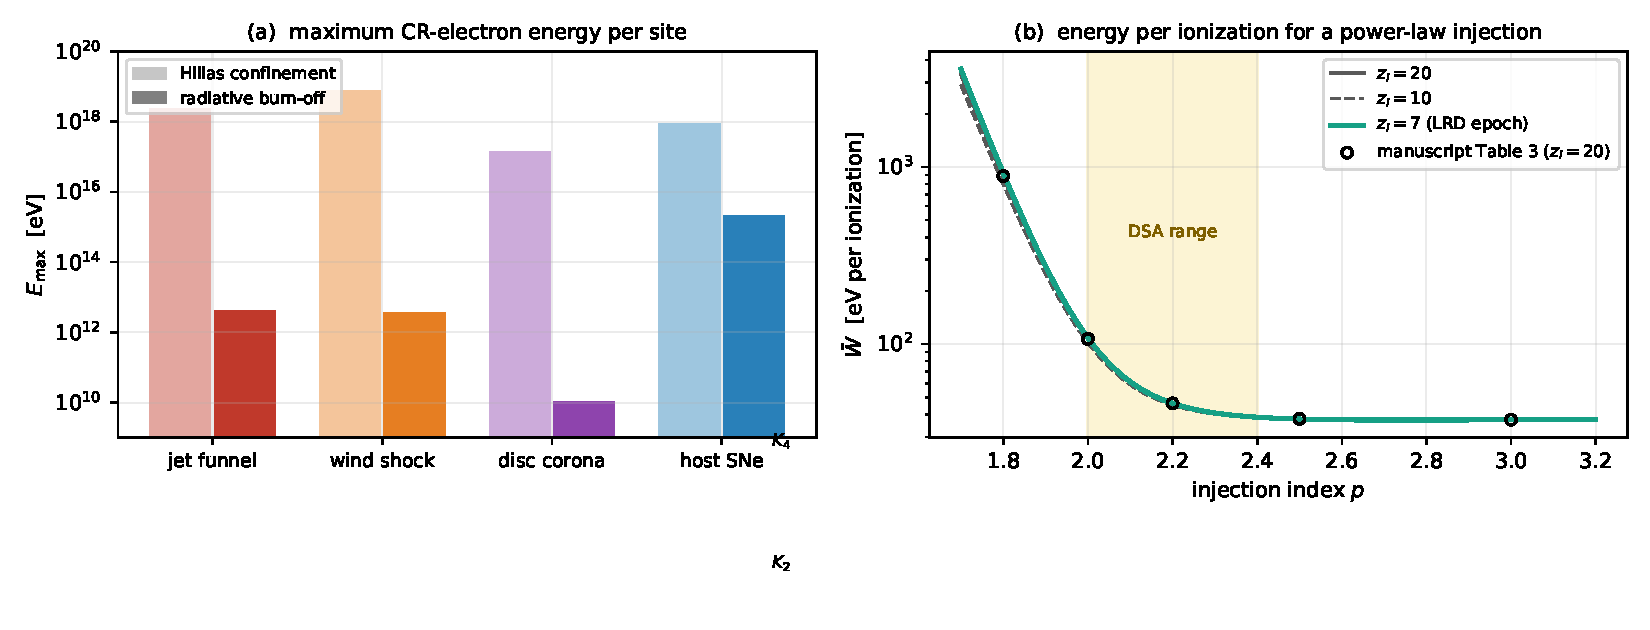
\includegraphics[width=\textwidth]{fig_lrd_cr.pdf}
\caption{\emph{(a)} Maximum cosmic-ray electron energy per site. Confinement
(Hillas, Eq.~\ref{eq:hillas}) is never the binding constraint; radiative
burn-off (Eq.~\ref{eq:burnoff}) always is, and in the corona it collapses to
$10\ \mathrm{GeV}$. Dotted and dashed lines mark $K_2$ and $K_4$, the regime
boundaries of the companion manuscript. \emph{(b)} Spectrum-averaged energy per
ionization $\bar W(p)$ from the cascade yield table, at the LRD epoch
($\zi=7$, green) and at the two redshifts tabulated in the manuscript. Open
circles are the published Table~3 values, reproduced here to $0.14\%$. The
shaded band is the DSA range $s=2.0$--$2.4$. Produced by
\texttt{make\_lrd\_figures.py}.}
\label{fig:main}
\end{figure}

Three results follow immediately.

\paragraph{The radio limits do not bite.} At $z=5$,
$D_L=4.77\times10^{4}\ \mathrm{Mpc}$, so the $11\ \mu\mathrm{Jy}$ VLASS
$3\sigma$ stack limit of \citet{Perger2025} corresponds to a rest-frame
$L_{1.4\,\mathrm{GHz}}\le1.0\times10^{25}\ \mathrm{W\,Hz^{-1}}$ (for
$\alpha=-0.7$) and, integrated over $0.1$--$100\ \mathrm{GHz}$, to
$L_{\mathrm{sync}}\le1.5\times10^{42}\ergs$, i.e.\ $0.15\%$ of $L_{\mathrm{bol}}$.
Applying Eq.~(\ref{eq:deboost}) with the wind-site value
$U_{\mathrm{rad}}/U_B=100$ gives $L_e\le1.6\times10^{44}\ergs$, or $0.16\,
L_{\mathrm{bol}}$; for the jet site the bound is $0.39\,L_{\mathrm{bol}}$. The
forward estimate of Sect.~\ref{sec:normA} with $\epsilon_e=0.01$ gives
$L_e=10^{41}\ergs$ (wind) to $4\times10^{42}\ergs$ (jet). \emph{The
observational bound is three orders of magnitude above the prediction.} The
radio silence of LRDs is therefore not evidence against a cosmic-ray electron
population; it is a statement about $U_B/U_{\mathrm{rad}}$, exactly as
\citet{Rodriguez2026} argue.

\paragraph{Neither do the X-ray limits, for a different reason.} The power that
does not emerge as synchrotron emerges as inverse Compton on the
$T\sim5000\ \mathrm{K}$ photospheric field \citep{Gentile2026}, whose peak is at
$1.2\ \mathrm{eV}$. For a cooled $s=2$ population the inverse-Compton continuum
is flat in $\nu F_\nu$ and spans $\simeq11.8$ decades from $6.5\ \mathrm{eV}$ to
the Klein--Nishina turnover, so $5.9\%$ of $L_e$ falls in $2$--$10\ \mathrm{keV}$.
The fiducial wind case gives $L_{2-10}=5.9\times10^{39}\ergs$, a factor $53$
below the stacked \emph{Chandra} limit $\log L_{2-10}\lesssim41.5$; an
aggressive jet case ($\epsilon_e=0.1$ of $L_{\mathrm{Edd}}$) gives
$2.3\times10^{42}\ergs$, a factor $7.5$ \emph{above} it. \textbf{[A]} My reading
is that this does not exclude the aggressive case, because the same
Compton-thick column ($N_{\mathrm H}=10^{24}$--$10^{25}\ \mathrm{cm^{-2}}$)
invoked to explain the X-ray weakness \citep{Tortosa2026,Pacucci2026} absorbs
the $2$--$10\ \mathrm{keV}$ band regardless of its origin. The conclusion is
that the cosmic-ray electron content of LRDs is at present observationally
\emph{unconstrained} from either side, and only the forward energetics and the
IGM consequences (Sect.~\ref{sec:igm}) can be used.

\paragraph{Escape.} A Compton-thick envelope has a grammage of
$1.7$--$17\ \mathrm{g\,cm^{-2}}$; at the minimum-ionizing rate of
$\sim\!2\ \mathrm{MeV\,(g\,cm^{-2})^{-1}}$ this stops electrons below roughly
$30$--$300\ \mathrm{MeV}$. Electrons above that traverse the envelope, so a
$\gamma_{\max}\sim10^{6}$ population loses only its low-energy end on the way
out. The escaping fraction $f_{\mathrm{esc}}^{\mathrm{CR}}$ into the IGM must
still be treated as a free parameter \textbf{[A]}, since it depends on the
magnetic topology of the host, which no LRD observation constrains.

% =====================================================================
\section{Closing the loop: what this delivers to the IGM}
\label{sec:igm}
% =====================================================================
The companion manuscript computes, for an electron injected at $\zi$ with
kinetic energy $\Kini$, the total number of ionizations $Y(\Kini,\zi)$ summed
over every generation of the cascade, and the spectrum-averaged energy per
ionization $\bar W$ for a power-law injection. Evaluating that machinery on the
$\zi=7$ row --- the lowest redshift at which the table is populated, and the
LRD epoch --- gives
\begin{equation}
  \bar W(\zi=7) = 925,\;108,\;46.3,\;37.7,\;37.4\ \mathrm{eV}
  \quad\text{for}\quad p=1.8,\;2.0,\;2.2,\;2.5,\;3.0 ,
\end{equation}
and the same code reproduces the published Table~3 values at $\zi=20$ and
$\zi=10$ to a maximum deviation of $0.14\%$ (Fig.~\ref{fig:main}b). For the
DSA index $s=2$ the relevant value is $\bar W=108\ \mathrm{eV}$. Note that
$p=1.8$ must \emph{not} be used here: for $p<2$ the integral is dominated by
$K_{\max}$, where the $\zi=7$ yields are truncated by the $z=5.5$ end of the
integration.

The comoving energy per hydrogen atom deposited by the LRD population is
\begin{equation}
  \varepsilon_{\mathrm H}
  = f_{\mathrm{esc}}^{\mathrm{CR}}\,
    \frac{n_{\mathrm{LRD}}\,L_e\,t_{\mathrm{era}}}{n_{\mathrm H}},
  \qquad
  \frac{N_{\mathrm{ion}}}{n_{\mathrm H}}=\frac{\varepsilon_{\mathrm H}}{\bar W},
  \qquad
  \Delta T = \frac{N_{\mathrm{ion}}}{n_{\mathrm H}}\times
             \bigl(4.3\text{--}6.9\bigr)\times10^{4}\ \mathrm{K},
  \label{eq:igm}
\end{equation}
the last relation being the heat--ionization lock derived in Sect.~9.4 of the
manuscript, inverted. With $n_{\mathrm H}=1.944\times10^{-7}\cmt$ comoving and
$t_{\mathrm{era}}=800\ \mathrm{Myr}$ ($z=7\to4$), Table~\ref{tab:igm} gives the
result.

\begin{table}[t]\centering\small
\caption{Cosmic-ray electron deposition in the IGM from the LRD population,
Eq.~(\ref{eq:igm}), with $\bar W=108\ \mathrm{eV}$. The last row is an
aggressive upper case ($\epsilon_e=0.1$ of the Eddington jet power, full escape,
high abundance) and is excluded by the measured thermal history.}
\label{tab:igm}
\begin{tabular}{@{}rrrrrl@{}}
\toprule
$n_{\mathrm{LRD}}$ [cMpc$^{-3}$] & $L_e$ [erg\,s$^{-1}$] &
$f_{\mathrm{esc}}^{\mathrm{CR}}$ & $\varepsilon_{\mathrm H}$ [eV] &
$N_{\mathrm{ion}}/n_{\mathrm H}$ & $\Delta T$ [K] \\
\midrule
$10^{-5}$ & $10^{41}$            & $0.1$ & $2.8\times10^{-4}$ & $2.6\times10^{-6}$ & $0.11$--$0.18$ \\
$10^{-5}$ & $10^{41}$            & $1$   & $2.8\times10^{-3}$ & $2.6\times10^{-5}$ & $1.1$--$1.8$ \\
$10^{-4}$ & $10^{41}$            & $1$   & $2.8\times10^{-2}$ & $2.6\times10^{-4}$ & $11$--$18$ \\
$10^{-5}$ & $4.0\times10^{43}$   & $0.1$ & $0.11$             & $1.0\times10^{-3}$ & $44$--$70$ \\
$10^{-4}$ & $4.0\times10^{43}$   & $1$   & $11.0$             & $0.10$             & $4400$--$7000$ \\
\bottomrule
\end{tabular}
\end{table}

Three readings of Table~\ref{tab:igm}. First, the realistic rows sit at
$N_{\mathrm{ion}}/n_{\mathrm H}\sim10^{-6}$--$10^{-4}$, one to three orders of
magnitude below the $2.3\times10^{-4}$--$4.6\times10^{-3}$ that the manuscript
obtains for the hadronic $\Delta T=10$--$200\ \mathrm{K}$ scale of
\citet{Leite2017}: LRDs are not a competitive ionizing source, and by the
argument of Sect.~9.4 of the manuscript their net effect on the photon budget
\citep{Munoz2024} is again to \emph{widen} it, by a negligible amount. Second,
the $\Delta T$ column is the interesting one, because $\Delta T\sim1$--$18\
\mathrm{K}$ is comparable to or above the adiabatic floor
$T_{\mathrm{ad}}(z=7)=1.33\ \mathrm{K}$, which is the regime the 21-cm
experiments are sensitive to: LOFAR disfavours mean gas temperatures below
$44\ \mathrm{K}$ at $z=9.1$ \citep{Mertens2025,Ghara2025} and HERA requires the
gas above the adiabatic floor by $z=10.4$ \citep{HERA2023}. Third, the last row
--- $\Delta T\sim5\times10^{3}\ \mathrm{K}$ --- would be flatly inconsistent
with the measured $T_0\simeq1.0$--$1.2\times10^{4}\ \mathrm{K}$ at
$z=5.4$--$5.8$ \citep{Gaikwad2020} for gas that is only then being photoheated,
and is therefore excluded. \textbf{[A]} That exclusion is itself a result: the
thermal history caps the product
$n_{\mathrm{LRD}}\,\epsilon_e\,f_{\mathrm{esc}}^{\mathrm{CR}}$, and it does so
far more tightly than any radio or X-ray stack.

% =====================================================================
\section{Verification}
\label{sec:ver}
% =====================================================================
\texttt{verify\_algebra.py} checks fifteen results with \textsc{SymPy}, each
by symbolic manipulation rather than numerical spot-checking: the strong-shock
compression ratio and Eq.~(\ref{eq:dsa}); Eq.~(\ref{eq:alpha}) by two
independent kernels; the cooling steepening of Eq.~(\ref{eq:cool}); the
normalization integral of Eq.~(\ref{eq:norm}) including the $s\to2$ limit; the
de-boosting factor of Eq.~(\ref{eq:deboost}); the K-correction exponent of
Eq.~(\ref{eq:kcorr}); the minimum-energy ratio of Eq.~(\ref{eq:equip}); the two
$E_{\max}$ expressions and the $B$-independence of Eq.~(\ref{eq:burnphot}); and
the internal consistency of Eq.~(\ref{eq:igm}) with the manuscript's lock. Unit
conversions are checked numerically: the Hillas prefactor evaluates to
$299.8\ \mathrm{eV\,G^{-1}\,cm^{-1}}$ and Eq.~(\ref{eq:burnphot}) to
$236.3\ \mathrm{MeV}$. \texttt{lrd\_cr\_numbers.py} reproduces Table~3 of the
manuscript to $0.14\%$ as an end-to-end regression on the figure and table
values generated previously.

% =====================================================================
\section{Summary}
% =====================================================================
\begin{enumerate}
\item Nine hypotheses for LRDs are alive as of August 2026
      (Table~\ref{tab:hyp}); the field has converged on a super-Eddington engine
      inside a dense, scattering-dominated envelope, with the mass of the engine
      ($10^{3}$--$10^{7}M_\odot$) and the geometry of the outflow the open
      questions.
\item Four of them contain a genuine cosmic-ray acceleration site: the polar
      jet funnel, the fast wind driving into the envelope, and (for the stellar
      readings) host supernovae. The disc corona is a heater, not an
      accelerator; the quasi-star and supermassive-star models have no
      supersonic converging flow at all.
\item The index follows from shock physics, $s=(r+2)/(r-1)\to2$, steepening to
      $s+1\simeq3$ above the cooling break; it must \emph{not} be read off the
      radio slope, which is optically thick in the one case where it has been
      measured. The normalization follows either from
      $L_e=\epsilon_e L_{\mathrm{mech}}$ or, as an upper bound, from the radio
      stacks corrected by $1+U_{\mathrm{rad}}/U_B$.
\item That correction factor is $10^{2}$--$10^{5}$, so the radio non-detections
      bound the electron power three orders of magnitude above the fiducial
      prediction. The X-ray stacks come within a factor of a few of the
      aggressive case but are evaded by the Compton-thick column. The tightest
      real constraint on the cosmic-ray electron output of LRDs is the measured
      IGM thermal history, through Eq.~(\ref{eq:igm}).
\end{enumerate}

% =====================================================================
\section{Publications cited, with online access}
\label{sec:refs}
% =====================================================================
\begingroup\small
\begin{longtable}{@{}p{0.30\textwidth}p{0.40\textwidth}p{0.24\textwidth}@{}}
\toprule
Reference & Cited for & Free access \\
\midrule \endhead
\multicolumn{3}{@{}l}{\textbf{Discovery and demographics}}\\
\citet{Matthee2024} & LRD definition; $n\sim10^{-5}$--$10^{-4}$ cMpc$^{-3}$ & \url{https://arxiv.org/abs/2306.05448}\\
\citet{Labbe2025} & candidate red AGN at $3<z<7$ & \url{https://arxiv.org/abs/2306.07320}\\
\citet{Greene2024} & spectroscopic confirmation of broad lines & \url{https://arxiv.org/abs/2309.05714}\\
\citet{Kocevski2025} & LRD sample in the JWST legacy fields & \url{https://arxiv.org/abs/2404.03576}\\
\citet{Akins2025} & COSMOS-Web overabundance; $R_{4400}\le10$ & \url{https://arxiv.org/abs/2406.10341}\\
\citet{Loiacono2026} & no number-density evolution at $z>2$ & \url{https://arxiv.org/abs/2606.30253}\\
\citet{Vaida2026} & 2026 mini-review of the competing scenarios & \url{https://arxiv.org/abs/2601.00089}\\
\addlinespace
\multicolumn{3}{@{}l}{\textbf{The nine hypotheses}}\\
\citet{Naidu2025} & black-hole star (H2) & \url{https://arxiv.org/abs/2503.16596}\\
\citet{Rusakov2026} & dense ionized cocoon, $M_{\rm BH}=10^{5-7}M_\odot$ (H3) & \url{https://arxiv.org/abs/2503.16595}\\
\citet{Barrufet2026} & LRD/LBD regimes support cocoon models (H3) & \url{https://arxiv.org/abs/2608.21522}\\
\citet{Liu2025} & Balmer break from super-Eddington accretion (H4) & \url{https://arxiv.org/abs/2507.07190}\\
\citet{LiuJR2026} & optically thick supercritical outflow (H4) & \url{https://arxiv.org/abs/2607.17448}\\
\citet{Zhou2026} & supermassive SS\,433 analogue (H5) & \url{https://arxiv.org/abs/2606.21105}\\
\citet{Naidu2026} & $\eta$\,Car / Type IIn engine; wind shocks (H6) & \url{https://arxiv.org/abs/2606.30711}\\
\citet{Pacucci2026} & direct-collapse black hole (H7) & \url{https://arxiv.org/abs/2601.14368}\\
\citet{Gentile2026} & quasi-star model; $T\sim5000$ K photosphere (H8) & \url{https://arxiv.org/abs/2606.06575}\\
\citet{AmaroSeoane2026} & nested supermassive star (H8) & \url{https://arxiv.org/abs/2607.20617}\\
\citet{Shi2026} & black-hole stars from star--BH collisions (H8) & \url{https://arxiv.org/abs/2608.27596}\\
\citet{Roy2026} & ultra-compact star-forming galaxies (H9) & \url{https://arxiv.org/abs/2606.23683}\\
\addlinespace
\multicolumn{3}{@{}l}{\textbf{X-ray and radio constraints}}\\
\citet{Ananna2024} & first X-ray view of LRDs & \url{https://arxiv.org/abs/2404.19010}\\
\citet{Sacchi2025} & 400 Ms \emph{Chandra} stack; non-detection & \url{https://arxiv.org/abs/2505.09669}\\
\citet{Tortosa2026} & X-ray weakness vs.\ local AGN; $N_{\rm H}$ & \url{https://arxiv.org/abs/2603.10162}\\
\citet{Perger2025} & 919 LRDs; $3\sigma$ of 11 and 18 $\mu$Jy\,beam$^{-1}$ & \url{https://arxiv.org/abs/2411.19518}\\
\citet{Mazzolari2026} & compilation of all radio stacks; SKAO forecast & \url{https://arxiv.org/abs/2606.30757}\\
\citet{Rodriguez2026} & radio-bright local analogue; IC radio dimming & \url{https://arxiv.org/abs/2608.16200}\\
\addlinespace
\multicolumn{3}{@{}l}{\textbf{Cosmic-ray physics and outflows}}\\
\citet{Kuze2026} & only explicit CR model of an LRD; jet funnel & \url{https://arxiv.org/abs/2601.11203}\\
\citet{Korber2026} & fast AGN-driven outflow, $L_{\rm kin}\sim10^{43}$ erg s$^{-1}$ & \url{https://arxiv.org/abs/2604.08687}\\
\citet{Bell1978} & diffusive shock acceleration & \url{https://ui.adsabs.harvard.edu/abs/1978MNRAS.182..147B}\\
\citet{BlandfordOstriker1978} & shock acceleration spectral index & \url{https://ui.adsabs.harvard.edu/abs/1978ApJ...221L..29B}\\
\citet{Drury1983} & DSA review; $s=(r+2)/(r-1)$ & \url{https://ui.adsabs.harvard.edu/abs/1983RPPh...46..973D}\\
\citet{Hillas1984} & confinement limit $E_{\max}=eBR\beta$ & \url{https://ui.adsabs.harvard.edu/abs/1984ARA\%26A..22..425H}\\
\citet{RybickiLightman1979} & synchrotron emissivity and $\alpha=-(s-1)/2$ & \url{https://ui.adsabs.harvard.edu/abs/1979rpa..book.....R}\\
\citet{Kellermann1989} & radio-loudness parameter $R_{4400}$ & \url{https://ui.adsabs.harvard.edu/abs/1989AJ.....98.1195K}\\
\citet{Novak2017} & SFR--radio luminosity calibration & \url{https://arxiv.org/abs/1703.09724}\\
\citet{Delvecchio2021} & $q_{\rm IR}(M_\star,z)$ infrared--radio correlation & \url{https://arxiv.org/abs/2101.06192}\\
\citet{Popesso2023} & star-forming main sequence & \url{https://arxiv.org/abs/2203.10487}\\
\addlinespace
\multicolumn{3}{@{}l}{\textbf{IGM and reionization context}}\\
\citet{Planck2020} & cosmology; $\sigma(\tau)=0.007$ & \url{https://arxiv.org/abs/1807.06209}\\
\citet{Leite2017} & $\Delta T=10$--$200$ K hadronic CR heating scale & \url{https://arxiv.org/abs/1703.09337}\\
\citet{HERA2023} & IGM above the adiabatic floor by $z=10.4$ & \url{https://arxiv.org/abs/2210.04912}\\
\citet{Mertens2025} & LOFAR power-spectrum upper limits & \url{https://arxiv.org/abs/2503.05576}\\
\citet{Ghara2025} & $\bar T<44$ K disfavoured at $z=9.1$ & \url{https://arxiv.org/abs/2505.00373}\\
\citet{Gaikwad2020} & $T_0\simeq1.0$--$1.2\times10^{4}$ K at $z=5.4$--$5.8$ & \url{https://arxiv.org/abs/2001.10018}\\
\citet{Munoz2024} & the photon budget crisis & \url{https://arxiv.org/abs/2404.07250}\\
\bottomrule
\end{longtable}
\endgroup

\bibliography{lrd_refs}
\end{document}
